\subsection{Unpipelined Design}
The first step in the project other than learning how to develop in Verilog was to create an unpipelined version of the intended processor.
This version is quite more simple than the pipelined version as it doesn't have to deal with the hazards that can occur in a pipelined and 
issues with branches and jumps but also because it doesn't need any pipeline registers in between the different stages. I will give you an 
overall view of the design without the details of each connection between the different modules since it is not the main focus of this project 
and was more of a way to learn how to use Verilog and the tools associated with it but also a temporary step before the pipelined version.

\begin{figure}[H]
    \centering
    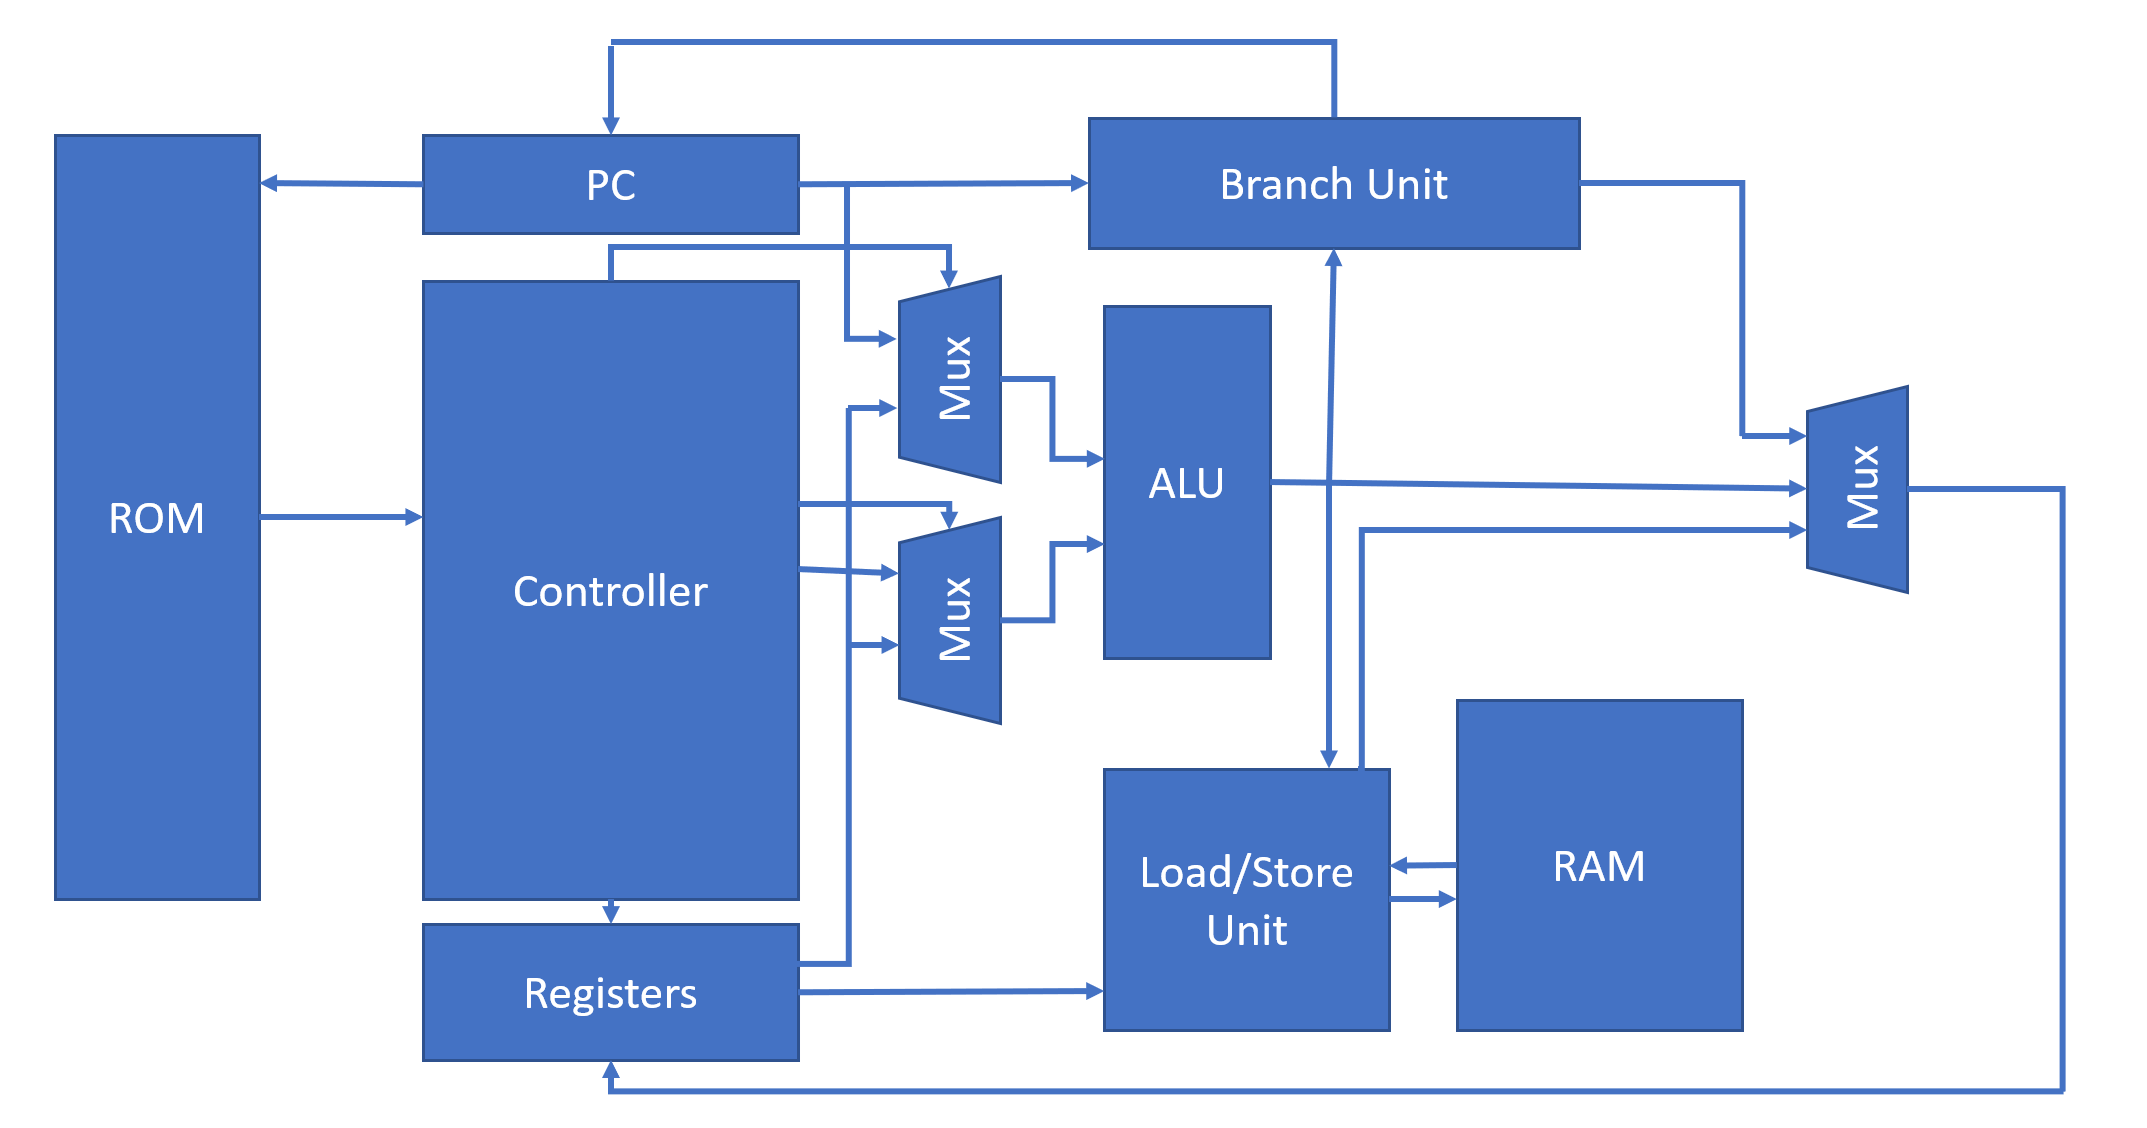
\includegraphics[width=0.85\textwidth]{design/unpipelined/images/unpipelined_cpu.png}
    \caption{Unpipelined CPU design}
    \label{fig:unpipelined_cpu_design}
\end{figure}

I will not go into the details of each module since it will be done in the next section about the pipelined version but I will give you a
brief overview of how the unpipelined version works.
First, the instruction is loaded from the ROM using the address given by the PC (Program Counter). Then the instruction needs to be decoded to know 
what it does and what are the operands and that's the job of the Controller that will try to match the different types of instruction to finally 
find the right one. Once it is done, it will output the different control signals to the register file, the ALU, the branch unit and the load/store unit such 
that it executes the instruction correctly with the correct data. The role of the ALU (Arithmetic Logic Unit) is to execute the different arithmetic
and logic operations such as addition, subtraction, multiplication, division, bitwise operations, etc. In the case of a branch instruction, the branch unit
will check if the instruction is a conditional one or not. In case it is one then it uses the result of the ALU to check if the condition is true or not
and update the PC accordingly. Finally, the load/store unit will load or store data from or to the RAM depending on the instruction. It is also using the 
result of the ALU since we can offset the address by an immediate value and that needs to be done by the ALU\@.
At the end of the cycle, a MUX will select among the three different results (ALU, branch unit and load/store unit) the one that will be written to the register file
according of course to the instruction executed.
Everything is done in one cycle and the next instruction is loaded from the ROM and the process starts again. \\

As we can see, the unpipelined version is quite simple then why do we need to pipeline it? The answer is performance. Indeed, the unpipelined version
is quite slow since it needs to wait for the instruction to be executed before loading the next one. But that can be improved by pipelining the processor
that will divide the execution of an instruction into multiple stages and execute multiple instructions at the same time and that's what we will see in the next section.

